%-------------------------------------------------------------------------------НЕ ПРОМЕНЯЙ!!!
%-------------------------------------------------------------------------------
\documentclass[12pt]{article}
%\usepackage[cp1251]{inputenc}
\usepackage[utf8]{inputenc}
\usepackage[bulgarian]{babel}
\usepackage{amssymb,amsmath,amsfonts,amstext,amscd,latexsym}
\usepackage{graphicx}
\usepackage[colorinlistoftodos]{todonotes}
\usepackage{systeme}
\usepackage{listings}
\usepackage{color}
\lstset{ 
	language=Matlab,                		% choose the language of the code
	%	basicstyle=10pt,       				% the size of the fonts that are used for the code
	numbers=left,                  			% where to put the line-numbers
	numberstyle=\footnotesize,      		% the size of the fonts that are used for the line-numbers
	stepnumber=1,                   			% the step between two line-numbers. If it's 1 each line will be numbered
	numbersep=5pt,                  		% how far the line-numbers are from the code
	%	backgroundcolor=\color{white},  	% choose the background color. You must add \usepackage{color}
	showspaces=false,               		% show spaces adding particular underscores
	showstringspaces=false,         		% underline spaces within strings
	showtabs=false,                 			% show tabs within strings adding particular underscores
	%	frame=single,	                			% adds a frame around the code
	%	tabsize=2,                				% sets default tabsize to 2 spaces
	%	captionpos=b,                   			% sets the caption-position to bottom
	breaklines=true,                			% sets automatic line breaking
	breakatwhitespace=false,        		% sets if automatic breaks should only happen at whitespace
	escapeinside={\%*}{*)}          		% if you want to add a comment within your code
}

\begin{document}
\begin{titlepage}	
	\newcommand{\HRule}{\rule{\linewidth}{0.5mm}} % Defines a new command for the horizontal lines, change thickness here
	\center % Center everything on the page
	\textsc{\LARGE Софийски университет "Св. Климент Охридски" }\\[0.3cm]
	\textsc{\Large Факултет по математика и информатика }\\[0.2cm]
	%\fontsize{size}{baselineskip}
	\HRule \\[0.8cm] {\fontsize{50}{80}\selectfont \bf П Р О Е К Т} \\[0.1cm] \HRule \\[1cm]
	{\fontsize{12}{18}\selectfont \bf ДИФЕРЕНЦИАЛНИ УРАВНЕНИЯ И ПРИЛОЖЕНИЯ}\vspace{15pt}\newline спец. Информатика, II курс, зимен семестър \newline учебна година 2021/2022 
	\vspace{30pt}
%-------------------------------------------------------------------------------НЕ ПРОМЕНЯЙ!!!
%-------------------------------------------------------------------------------
		
		
		
		\begin{minipage}{0.4\textwidth}
			\begin{flushleft}\large
				\emph{Изготвил:} \\
				Теодор Христов \\ 
				фак. номер 45799 \\ 
				група: 4 %Попълнете вашето име, факултетен номер и група.
			\end{flushleft}
		\end{minipage}
		~
		%\begin{flushleft}
		\begin{minipage}{0.4\textwidth}
			\begin{flushright}
				\large
				\emph{Дата:}\\
				20. 01.  2022г. % Попълнете датата на предаване
				\\София 
			\end{flushright}
		\end{minipage}\\[1cm]
		%\end{flushleft}
		\bigskip
		{\large \textbf{Тема \textnumero 53}}\\[1cm] % Date, change the \today to a set date if you want to be precise
		%
\includegraphics{rsz_sofia_university_logo.png}\\[1cm] 
		
\includegraphics{logo_su_no_text.png}\\[1cm]
		\vfill % Fill the rest of the page with whitespace
\end{titlepage}
\tableofcontents
\newpage
\section{Задание на проекта}
\begin{enumerate}
	\item Да се начертаят, с червен цвят, графиките на първите 5 последователни приближения на решението на задачата на Коши $$xdy=-2ydx,\quad y(2)=1$$ в интервала $[1,10]$, получени по метода на Пикар. В същата фигура да се начертае със син цвят графиката на точното решение на задачата на Коши, което да се извежда в командния прозорец. Да се опишат в легенда съответните линии на чертежа.
\end{enumerate}
\newpage
\section{Решение на задача 1}
\subsection{Теоретична обосновка}
Задача на Коши за диференциално уравнение от вида $y'=f(x,y)$ се нарича задачата за намиране на решение на уравнението, което удовлетворява условието $y(x_0)=y_0$ (начално условие), където точката $(x_0,y_0)$ е от дефиниционното множество на функцията $f$. При определени условия за функцията $f$, задачата на Коши има единствено решение, дефинирано в околност на $x_0$, което може да се определи по различни начини. Един от тях е метода на Пикар (Picard). Накрадко метода се свежда до намиране на нови функции, които се получават по следния начин:

Нека за целта на примера $y(t) = \tan(t)$, решението на уравнението $y\prime(t) = 1 + y(t)^2$ с начално условие $y(t_0) = y_0 = 0$. Започвайки от $\phi_0(t) = 0$ итерираме и получаваме:$\newline$


$\phi_1(t) = \int_{0}^{t} (1+0^2) \,ds = t\newline$

$\phi_2(t) = \int_{0}^{t} (1+s^2) \,ds = t + \dfrac{t^3}{3}\newline$

$\phi_3(t) = \int_{0}^{t} (1+(s + \dfrac{s^3}{3})^2 \,ds = t + \dfrac{t^3}{3} + \dfrac{2t^5}{15} + \dfrac{t^7}{63}\newline$

И така получаваме $\phi_n(t) \rightarrow y(t).\newline$

По същество в задачата се иска да се начертаят графиките на няколко функции, които се извеждат по метода на Пикар. 
\subsection{MATLAB код}
Описание на програмната реализация. Задаваме наименования на осите, след това задаваме интервала, в който трябва да работим. Използваме \textit{dsolve} за да сметнем диференциалното уравнение след което изчертаваме точното решение на задачата на Коши дадена в условието Приближенията на функцията дадена в условието получаваме, като задаваме началните условия от условието и броя приближения които искаме да направим, след това по дефиницията на метода на Пикар итерираме и получаваме приближенията.
\lstinputlisting[language=Matlab]{Task1_45799.m}%!!!!файлът Eulertest.m трябва да се съдържа в папката temaNN_FakNomer 
\subsection{Резултати} На фигурата са изобразени с различни цветове точното решение, както и 5 приближения на решението на задачата получени по метода на Пикар. Формула за точното решение се извежда на екрана в командния прозорец. От графиките на фигурата виждаме, че с всяко следващо приближение, разликата между точното решение и съответното приближено решение става все по-малка. 
\begin{figure}
	\centering
	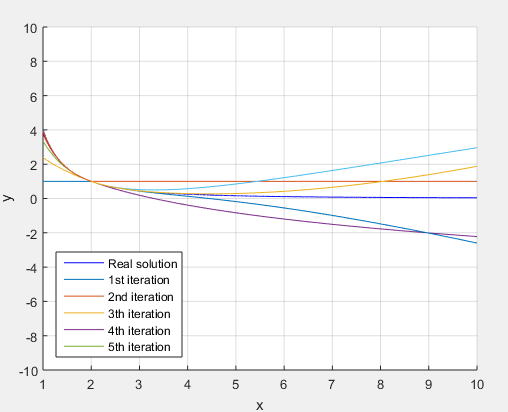
\includegraphics{5pikar.png}%{Figure name without .eps extension}
	\caption{Точното решение и приближенията му}
\end{figure} 
\begin{figure}
	\centering
	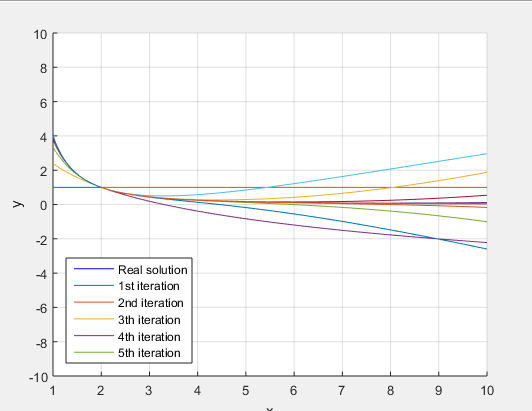
\includegraphics{50pikar.png}%{Figure name without .eps extension}
	\caption{Точното решение и 50 приближения}
\end{figure} 
\end{document}